\documentclass[11pt]{article}
% Shared preamble for main.tex and supplementary.tex.
% --- page and typography ---
\usepackage[a4paper,margin=1in]{geometry}
\usepackage{microtype}
\usepackage[T1]{fontenc}
\usepackage{lmodern}
\linespread{1.05}

% --- math, units, figures, tables ---
\usepackage{amsmath}
\usepackage{siunitx}
\sisetup{detect-all, range-phrase={\text{--}}, range-units=single}
\usepackage{graphicx}
\graphicspath{{figures/}{../figures/}}
\usepackage{booktabs}
\usepackage[font=small,labelfont=bf]{caption}
\usepackage{placeins}

% --- references ---
\usepackage[backend=biber,style=numeric-comp,sorting=none,giveninits=true,maxbibnames=8,doi=true,url=false,isbn=false]{biblatex}
\addbibresource{references.bib}

% --- links and cross-refs (xr-hyper before hyperref, cleveref last) ---
\usepackage{xr-hyper}
\usepackage[hidelinks]{hyperref}
\usepackage[capitalise,nameinlink]{cleveref}

% Scrub PDF document properties so metadata stays anonymous for the EJP
% double-anonymous build (harmless in the named build).
\hypersetup{pdfauthor={},pdfsubject={},pdfkeywords={}}

% Reusable notation. Keep small; do not over-abstract.
\newcommand{\LD}{\textit{L/D}}
\newcommand{\ms}{\,\unit{\meter\per\second}}
\newcommand{\degr}{^{\circ}}
\newcommand{\cgfrac}{x_\mathrm{cg}}
\newcommand{\npfrac}{x_\mathrm{np}}

% numbers.tex: generated by analysis/export_numbers.py from metrics.json.
% Do not edit by hand; rerun the pipeline.

\newcommand{\nRelief}{10.2}
\newcommand{\nAspect}{230}
\newcommand{\nSlopeMean}{5.2}
\newcommand{\nSlopePninety}{12.8}
\newcommand{\nSlopeRadius}{400}
\newcommand{\nLiftIntoWind}{40}
\newcommand{\nLiftAlongSlope}{192}
\newcommand{\nContour}{5.1}
\newcommand{\nValleyDrop}{9.2}
\newcommand{\nHours}{175\,320}
\newcommand{\nFavPct}{15.6}
\newcommand{\nFavLo}{14.3}
\newcommand{\nFavHi}{17.0}
\newcommand{\nFavHours}{1\,370}
\newcommand{\nFavWinter}{21.1}
\newcommand{\nSWAnyPct}{34.3}
\newcommand{\nSWSixPct}{10.3}
\newcommand{\nSWSixHours}{906}
\newcommand{\nSWEightPct}{3.4}
\newcommand{\nSWEightLo}{2.9}
\newcommand{\nSWEightHi}{3.9}
\newcommand{\nSWEightHours}{296}
\newcommand{\nRidgePeak}{1.5}
\newcommand{\nRidgeWind}{8}
\newcommand{\nRidgeFormula}{1.8}
\newcommand{\nSinkBest}{1.9}
\newcommand{\nSinkNominal}{3.1}
\newcommand{\nRidgeMatchWind}{10}
\newcommand{\nTrimSpeed}{15.1}
\newcommand{\nMass}{80}
\newcommand{\nArea}{7}
\newcommand{\nCLtrim}{0.8}
\newcommand{\nTower}{18}
\newcommand{\nJump}{2}
\newcommand{\nHeightToTrim}{11.5}
\newcommand{\nLDStillSteady}{11.1}
\newcommand{\nStillRangeBest}{14}
\newcommand{\nStillRangeSteady}{142}
\newcommand{\nMaxRangeInto}{110}
\newcommand{\nMinWindBest}{5.7}
\newcommand{\nMinWindNominal}{10.6}
\newcommand{\nRangeEightBest}{271}
\newcommand{\nRangeEightNominal}{111}
\newcommand{\nRangeEightIntoBest}{104}
\newcommand{\nMinWindTowerLo}{6.6}
\newcommand{\nMinWindTowerHi}{3.8}
\newcommand{\nARlo}{3}
\newcommand{\nARhi}{5}
\newcommand{\nElo}{0.6}
\newcommand{\nEhi}{0.8}
\newcommand{\nCDzlo}{0.05}
\newcommand{\nCDzhi}{0.15}
\newcommand{\nLDlo}{3.1}
\newcommand{\nLDhi}{7.9}
\newcommand{\nLDnom}{4.7}
\newcommand{\nNPnotail}{0.25}
\newcommand{\nNPtail}{0.53}
\newcommand{\nCGlo}{0.35}
\newcommand{\nCGhi}{0.55}
\newcommand{\nCGonset}{0.30}
\newcommand{\nTloss}{0.74}
\newcommand{\nTdoubleRep}{0.24}
\newcommand{\nTdoubleFwd}{0.60}
\newcommand{\nTdoubleAft}{0.16}
\newcommand{\nTdoubleInLo}{0.12}
\newcommand{\nTdoubleInHi}{0.89}
\newcommand{\nFlightTime}{16}
\newcommand{\nReactLo}{0.15}
\newcommand{\nReactHi}{0.3}
\newcommand{\nSamples}{40\,000}
\newcommand{\nReachSlope}{6.9}
\newcommand{\nReachSlopeLo}{6.6}
\newcommand{\nReachSlopeHi}{7.1}
\newcommand{\nReachSlopeN}{2\,748}
\newcommand{\nReachInto}{0}
\newcommand{\nReachIntoHi}{0.01}
\newcommand{\nMedRangeSlope}{83}
\newcommand{\nMedRangeInto}{62}
\newcommand{\nNinetyRangeSlope}{180}
\newcommand{\nShortFifty}{34}
\newcommand{\nMedWindReach}{7.6}
\newcommand{\nTenWindReach}{5.4}
\newcommand{\nMedLDReach}{5.8}
\newcommand{\nMedLDAll}{4.7}
\newcommand{\nMedFlightReach}{24}
\newcommand{\nTdoubleMC}{0.29}
\newcommand{\nTdoubleMCpnn}{1.6}
\newcommand{\nTibiaLo}{7.5}
\newcommand{\nTibiaHi}{11.3}
\newcommand{\nOnsetMid}{9.7}
\newcommand{\nOnsetLo}{6.1}
\newcommand{\nOnsetHi}{14.1}
\newcommand{\nCtrlVzMed}{2.2}
\newcommand{\nCtrlVzMax}{4.1}
\newcommand{\nDepVzMed}{10.1}
\newcommand{\nDepAngLo}{35}
\newcommand{\nDepAngHi}{70}
\newcommand{\nVreachLo}{10.3}
\newcommand{\nVreachHi}{19.4}
\newcommand{\nPbreakDep}{58}
\newcommand{\nDecelG}{26}
\newcommand{\nExSinkNom}{3.1}
\newcommand{\nExUsoarNom}{14.2}
\newcommand{\nExSinkHi}{1.9}
\newcommand{\nExUsoarHi}{8.5}
\newcommand{\nExWilsonHalf}{0.25}
\newcommand{\nExHeadwind}{13.1}
\newcommand{\nExVdepFifty}{11.6}


\hypersetup{pdftitle={Supplementary material: Wind, slope, and the want of a tail}}
% Figures, tables, equations, and sections of the main text are labelled in main.tex.
\externaldocument{main}

\renewcommand{\thefigure}{S\arabic{figure}}
\renewcommand{\thetable}{S\arabic{table}}

\title{\bfseries Supplementary material for\\
Wind, slope, and the want of a tail:\\
a computational feasibility study of Eilmer of Malmesbury's flight}
\author{}
\date{}

\begin{document}
\maketitle

\noindent
This supplement gives the source extracts behind the historical and biomechanical
inputs (S1), the parameter ranges sampled in the Monte Carlo (S2), the ridge-lift field
(S3), and worked answers to the exercises of Section~6 of the main text (S4).
Figure, table, and equation numbers without an S refer to the main text.

\subsection*{S1. Source extracts}

\paragraph{S1.1 The flight, the distance, the injury, and the tail.}
The account is one passage of William of Malmesbury, \textit{Gesta Regum Anglorum}
(book II, ch.~225), in the Oxford Medieval Texts edition
\autocite{williamMalmesbury_gesta}:

\begin{quote}\small\itshape
Is erat litteris, quantum ad id temporis, bene imbutus, aeuo maturus, immanem
audaciam prima iuuentute conatus: nam pennas manibus et pedibus haud scio qua
innexuerat arte, ut Daedali more uolaret, fabulam pro uero amplexus, collectaque e
summo turris aura, spatio stadii et plus uolauit; sed uenti et turbinis uiolentia,
simul et temerarii facti conscientia, tremulus cecidit, perpetuo post haec debilis,
et crura effractus. Ipse ferebat causam ruinae quod caudam in posteriori parte
oblitus fuerit.
\end{quote}

\noindent In the standard English rendering:

\begin{quote}\small
He had by some means, I scarcely know what, fastened wings to his hands and feet so
that, mistaking fable for truth, he might fly like Daedalus, and, collecting the
breeze on the summit of a tower, he flew for more than the distance of a furlong.
But, agitated by the violence of the wind and the swirling of air, as well as by
awareness of his rashness, he fell, broke his legs, and was lame ever after. He
himself used to say that the cause of his failure was his forgetting to put a tail
on the back part.
\end{quote}

\noindent The distance is a \textit{stadium}, a furlong, about \SI{\nTarget}{\meter}.

\paragraph{S1.2 The tibia fracture threshold.}
The \SIrange{\nTibiaLo}{\nTibiaHi}{\kilo\newton} per-leg range in \cref{fig:biomech}
follows a systematic review \autocite{abidin2026tibia}, which reports that

\begin{quote}\small
tibial fracture thresholds range from \(\sim\)7.5 kN in female specimens to 11.3 kN
under combined axial and bending loads, with fibula contribution increasing axial
tolerance by \(\sim\)10\%.
\end{quote}

\noindent The upper figure traces to \textcite{salzar2014leg}, who recommend a tibial axial
threshold of about \SI{\nTibiaSalzar}{\kilo\newton}, rising to about \SI{\nTibiaHi}{\kilo\newton} with
the fibula.

\paragraph{S1.3 The medieval wind regime.}
\textcite{trouet2009nao} report

\begin{quote}\small
a 947-year-long multidecadal North Atlantic Oscillation (NAO) reconstruction [with]
a persistent positive NAO during the MCA [Medieval Climate Anomaly].
\end{quote}

\noindent \textcite{ortega2015nao} revise this, finding

\begin{quote}\small
no persistent positive NAO during the medieval period, but [suggesting] that
positive phases were dominant during the thirteenth and fourteenth centuries.
\end{quote}

\noindent Neither reconstruction indicates the weak westerlies of a persistent negative NAO
in the eleventh century, so the modern wind statistics are not taken to overstate
Eilmer's.
The analysis does not assume that medieval winds were stronger.

\subsection*{S2. Sampled parameter ranges}

\begin{table}[ht]
  \centering
  \caption{\textbf{Ranges sampled in the Monte Carlo (\cref{fig:montecarlo}).}
  All are uniform.
  The glide ratio is not sampled; it follows from aspect ratio, span efficiency, and
  zero-lift drag through \cref{eq:polar} and spans \numrange{\nLDlo}{\nLDhi}.
  The launch wind is drawn from the ERA5 southwest-sector hours at
  \SIrange{\nWindLo}{\nWindHi}{\meter\per\second}.}
  \label{tab:priors}
  \small
  \begin{tabular}{lll}
    \toprule
    Parameter & Range & Basis \\
    \midrule
    Wing area & \SIrange{\nAreaLo}{\nAreaHi}{\meter\squared} & wing spanning hands to feet \\
    All-up mass & \SIrange{\nMassLo}{\nMassHi}{\kilogram} & adult man and a timber frame \\
    Trim lift coefficient \(C_L\) & \numrange{\nCLlo}{\nCLhi} & cambered membrane \autocite{hoerner1985lift} \\
    Aspect ratio \(A\) & \numrange{\nARlo}{\nARhi} & span of one to two arm spans \\
    Span efficiency \(e\) & \numrange{\nElo}{\nEhi} & untwisted, non-elliptical wing \autocite{drela2014flight} \\
    Zero-lift drag \(C_{D0}\) & \numrange{\nCDzlo}{\nCDzhi} & membrane, prone body, frame \autocite{hoerner1965drag,lissaman1983lowre} \\
    Tower height & \SIrange{\nTowerLo}{\nTowerHi}{\meter} & around White's \SI{\nTower}{\meter} \autocite{white1961eilmer} \\
    Slope angle \(\theta_s\) & \ang{\nSlopeLo}--\ang{\nSlopeHi} & DEM 90th percentile as a floor \\
    Lift efficiency \(\eta\) & \numrange{\nEtaLo}{\nEtaHi} & flow following the surface \\
    CG \(\cgfrac\) & \numrange{\nCGlo}{\nCGhi}\,\(c\) & hands at leading edge, feet at trailing edge \\
    Neutral-point shift from a tail & \numrange{\nTailShiftLo}{\nTailShiftHi}\,\(c\) & tail size \\
    \bottomrule
  \end{tabular}
\end{table}

\FloatBarrier
\subsection*{S3. Ridge-lift field}

\begin{figure}[ht]
  \centering
  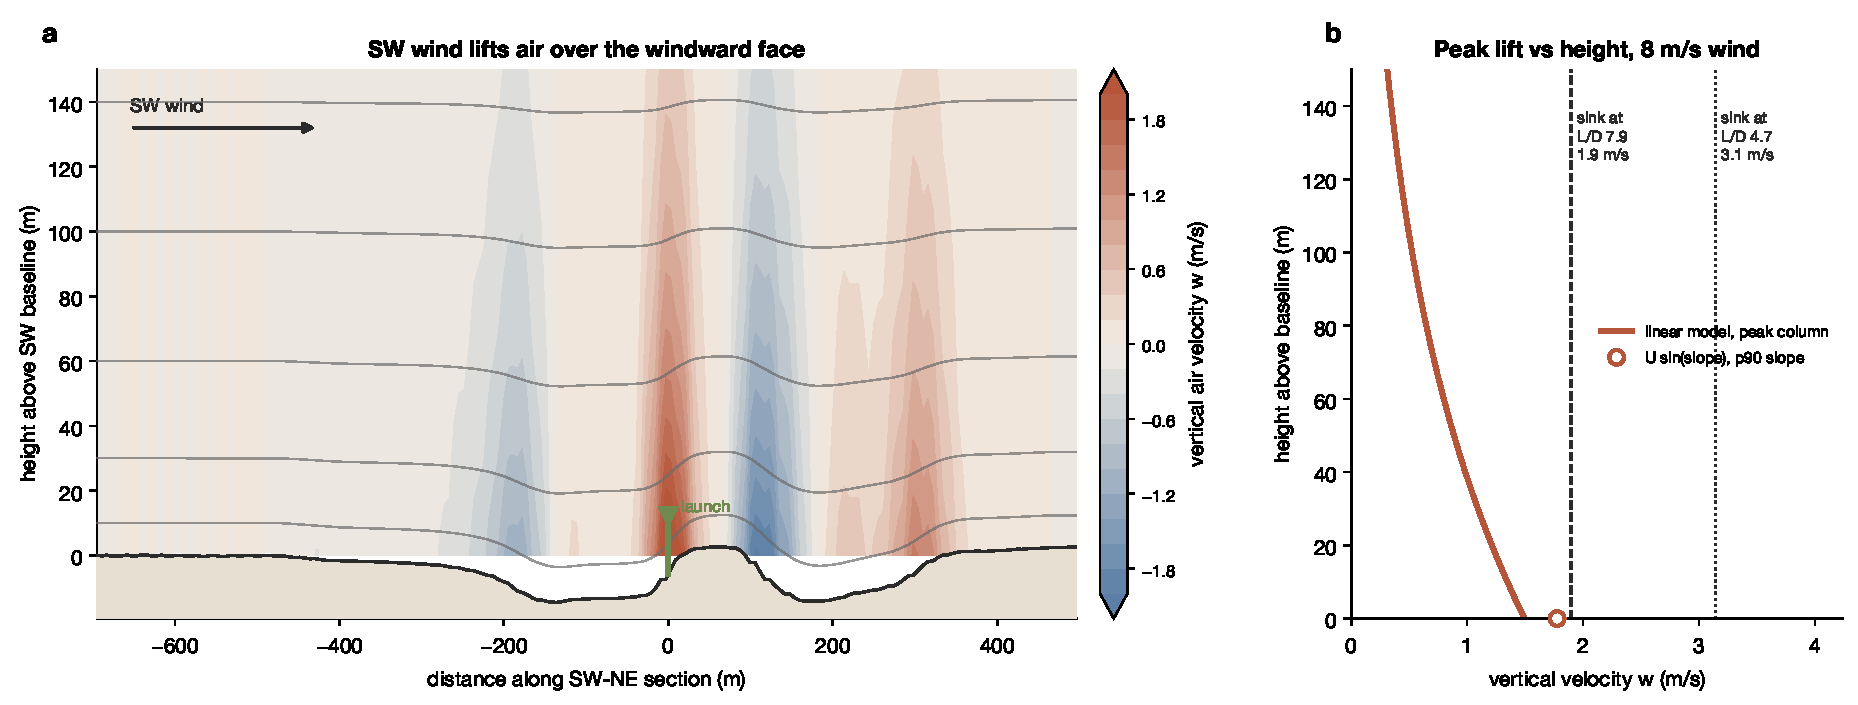
\includegraphics[width=\linewidth]{fig3_ridge_lift}
  \caption{\textbf{Ridge lift over the abbey spur.}
  The linear model of \cref{eq:ridge} over the measured southwest--northeast section.
  \textbf{(a)} Vertical air velocity and streamlines in an
  \SI{\nRidgeWind}{\meter\per\second} southwest wind.
  \textbf{(b)} Vertical air velocity against height above the point of strongest lift,
  \SI{\nRidgePeak}{\meter\per\second} at the surface.
  The open circle is the surface estimate \(U\sin\theta_s\) used in the glide model at the
  90th-percentile slope.
  The vertical lines are the still-air sink of the nominal craft at the highest and central
  glide ratios.}
  \label{fig:ridge}
\end{figure}

\FloatBarrier
\subsection*{S4. Answers to the exercises}

\paragraph{1. Energy at launch.}
Energy conservation gives \(\Delta h = (V^2 - v_0^2)/2g = \SI{\nHeightToTrim}{\meter}\), most
of an \SI{\nTower}{\meter} tower.
A headwind of \(V - v_0 \approx \SI{\nExHeadwind}{\meter\per\second}\) gives the full airspeed
at release.
The steady-glide estimate for the best wing is \(H\,(\LD) \approx
\SI{\nStillRangeSteady}{\meter}\); integrating \cref{eq:eom} gives
\SI{\nStillRangeBest}{\meter}, because the craft spends its height on the dive and the
pull-out.

\paragraph{2. Glide ratio.}
Minimising \(C_D/C_L\) with \(C_D = C_{D0} + C_L^2/(\pi e A)\) gives \(C_L^2 = \pi e A C_{D0}\),
at which the two drag terms are equal and \(\LD = \frac{1}{2}\sqrt{\pi e A/C_{D0}}\).
The corners of \cref{tab:priors} give \numrange{\nLDlo}{\nLDhi}.
\(C_{D0}\) varies by a factor of three and moves \LD\ by \(\sqrt{3}\), more than \(A\) or \(e\);
a drag measurement on a model of the wing and body would narrow it most.

\paragraph{3. Velocity triangles.}
Heading into the wind, the air and wind velocities are collinear and the ground speed is
\(V - U\).
Crabbing along a track perpendicular to the wind, the heading component into the wind must
equal \(U\), leaving \(\sqrt{V^2 - U^2}\) along the track.
The headwind adds to the airspeed at release on the first track, but subtracts from the
ground speed for the whole flight.

\paragraph{4. Ridge lift and sink.}
The sink rates are \SI{\nExSinkNom}{\meter\per\second} at \LD~\num{\nLDnom} and
\SI{\nExSinkHi}{\meter\per\second} at \LD~\num{\nLDhi}.
On a slope of \ang{\nSlopePninety} the lift matches them at \(U \approx
\SI{\nExUsoarNom}{\meter\per\second}\) and \SI{\nExUsoarHi}{\meter\per\second}.
Southwest winds of \SI{\nSWStrong}{\meter\per\second} or more occur in \SI{\nSWEightPct}{\percent} of
hours.
The full simulation needs less wind (\SI{\nMinWindBest}{\meter\per\second} for the best wing)
because the tower height covers part of the sink.

\paragraph{5. Pitch stability.}
With state \((\alpha, q)\), the matrix \(\begin{pmatrix} Z_\alpha & 1 \\ M_\alpha & M_q
\end{pmatrix}\) has a positive real eigenvalue when its determinant \(Z_\alpha M_q -
M_\alpha\) is negative, that is, when \(M_\alpha > Z_\alpha M_q\).
Since \(M_\alpha \propto \cgfrac - \npfrac\) and \(Z_\alpha M_q > 0\), divergence begins
slightly aft of the neutral point, at \num{\nCGonset}\,\(c\) for the nominal craft.
At \(\cgfrac = \nCGrep\), \(t_2 = \SI{\nTdoubleRep}{\second}\).
A ruler-drop test usually gives a simple reaction time of about \SI{\nRulerDrop}{\second}, so the
disturbance doubles about once per reaction.

\paragraph{6. Monte Carlo.}
For \(k = \nReachSlopeN\) and \(n = \nSamples\), \(\hat p = \SI{\nReachSlope}{\percent}\) and
the Wilson half-width is close to \(\nWilsonZ\sqrt{\hat p(1-\hat p)/n} \approx
\SI{\nExWilsonHalf}{\percent}\), giving \SIrange{\nReachSlopeLo}{\nReachSlopeHi}{\percent}.
Another seed changes the fraction by about this amount.

\paragraph{7. Impact.}
The onset speeds are \SIrange{\nOnsetLo}{\nOnsetHi}{\meter\per\second}.
At \(V = \SI{\nTrimSpeed}{\meter\per\second}\) and \ang{\nExDiveAngle}, the vertical speed is
\SI{\nExVdepFifty}{\meter\per\second}, above the onset speed for the central stopping
distance.
A glide into the ground at the sink rate, \SIrange{\nExSinkHi}{\nExSinkNom}{\meter\per\second},
is not.
The injury implies a steep, fast arrival, consistent with a loss of control but not proof
of one.


\printbibliography

\end{document}
